\subsection{Эксперимент 6.  Лучший алгоритм. Анализ ошибок алгоритма.}
\subsubsection{Дизайн эксперимента}
В ходе данного эксперимента брались лучшие параметры, подобранные на предыдущих шагах и лучший из разобранных алгоритмов (SGD):
\begin{enumerate}
	\item $\alpha = 0.1$
	\item  $\beta = 0.0347$
	\item  $\omega_0 = 0 \in \mathbb{R}^D$
	\item  $batch\_size = 10000 $
	\item Текст подвергался лемматизации и выкидыванию стоп-слов
	\item Использовалась модель векторизации BagOfWords
	\item $min\_df = 0.0001$
	\item $max\_df = 0.1$
	\item $max\_iters = 1000$ (для увеличения точности)
\end{enumerate}
В этом эксперименте в качестве обучающей и тестовой были взяты исходные данные, то есть никакого деления на валидационную выборку уже не происходило. После обучения на обучающей выборке была построена и проанализирована матрица ошибок предсказания на тестовых ответах. Также были разобраны типичные ошибки алгоритма на примерах.
\newpage
\subsubsection{Результаты эксперимента}
\begin{figure}[h]
	\caption{\centering Матрица ошибок}
	\centering{
	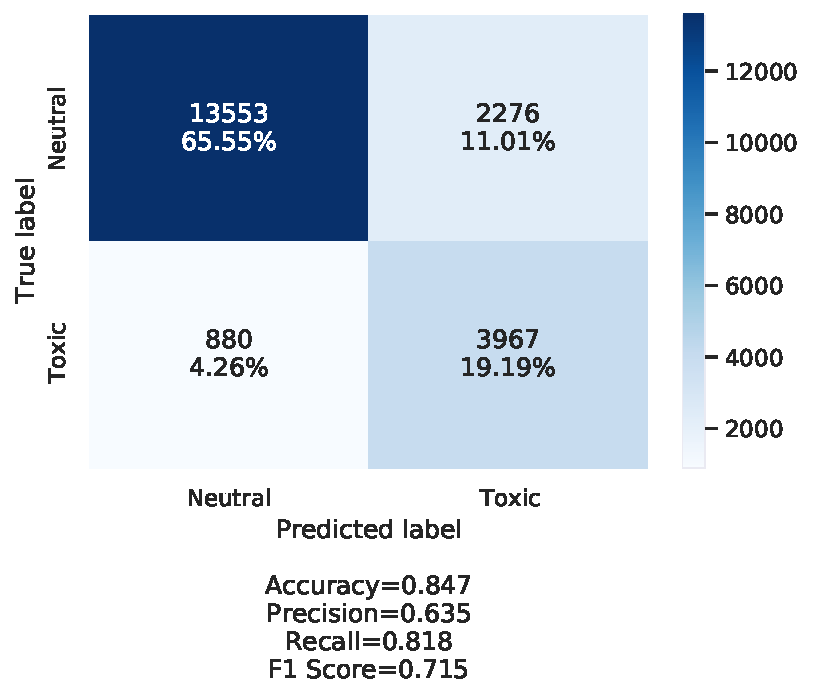
\includegraphics[width=0.7\linewidth]{conf_m.pdf}
	}
	\label{eq:confm}
\end{figure}
Как видим из рис.\ref{eq:confm} следует, что модель хорошо классифицирует
тексты, однако все же делает ошибки и чаще всего при классификации нейтральных текстов как токсичных. Рассмотри примеры текстов, на которых алгоритм чаще всего ошибается:\\
\begin{itemize}
	\item {\itshape "i think the origin of sagging has his roots in that human stupidity has no limits"{}, "alex  think again  mr  obama is the us  president  what about putin and his background  worse than an ass"{}} \\-- эти предложения были классифицированы, как нейтральные, хотя не являются такими. Вероятно, это происходит из-за того, что в этих текстах большая часть слов по-отдельности (кроме "stupidity" и "ass") это вполне обычные слова, употребляемые и в нейтральных текстах. \\
	\item "she looks like a horse" {} -- {}"horse" \ редко употребляется в качестве оскорбления, поэтому не верно классифицирован как нейтральный 
	\item "f u c k e r c o m m i e"{} -- из-за того, что есть пробельные слова это предложение будет представлено в виде вектора букв, а не слова. Понятно, что модель будет давать плохое предсказание, так как буквы не слова.
	\item {\itshape "we got snow here in boston  too    flying home tomorrow is going to suck"{}, "racism in moby dick       was herman melville a racist   particularly chapter 42 of moby dick  melville expounds on the terrifying aspects of the color white  how white dominates other colors  and how the white race dominates other races   was moby dick  the white whale  a symbol of white superiority and pride   i was shocked when i read this statement from chapter 42 pg  163 norton   1967  speaking on whiteness  melville writes       and though this preeminence in it applies to the human race itself  giving the white man mastership over every dusky tribe"{}}\\- тексты неверно классифицированы как токсичные. Алгоритм, ошибается, поскольку,  модель не знает контекст, и ошибочно воспринимает такие слова как "suck"\  и "dick"\  в "moby dick"\  как токсичные.
\end{itemize}
\subsubsection{Выводы эксперимента}
Таким образом, в основном алгоритм ошибается, поскольку не знает контекста, хотя бывает и в следствие наличия в текстовых данных данных, которые с формальной точки зрения не являются текстами (то есть непустой последовательностью, состоящей из слов, а не букв)